%!TEX root = ../main.tex

\chapter{Impianti}
\label{chp:impianti}
Nel capitolo precedente sono state elencate e brevemente introdotte le varie fonti energetiche che abbiamo a disposizione, sarà obbiettivo di questo capitolo elencare ed illustrare il funzionamento degli impianti utilizzabili per convertire le varie fonti energetiche in energia elettrica la quale sarà poi immessa nella rete elettrica.\\
\section{Impianto fotovoltaico}
Un'impianto fotovoltaico è un'impianto elettrico formato da più moduli fotovoltaici i quali, sfruttando l'energia solare, producono energia elettrica mediante appunto l'effetto fotovoltaico.\\
Si all'interno di un'impianto fotovoltaico possiamo identificare alcuni elementi chiave e fondamentali quali:
\begin{itemize}
    \item Cavi, diodi e magnetotermici
    \item Inverter
\end{itemize}
I primi elementi sono fondamentali per la connessione e la sicurezza dell'impianto mentre il secondo è necessario per la conversione DC-AC per poi poter immettere in rete l'energia elettrica che si produce.\\
Per illustrare il funzionamento di un'impianto è importante prima capire il funzionamento dell'effetto fotovoltaico.\\
\subsection{Effetto fotovoltaico}
Durante lo studio delle onde elettromagnetiche si notò come una radiazione elettromagnetica che investe un materiale possa, in certe condizioni, cedere energia agli elettroni più esterni degli atomi del materiale stesso.Se l'energia risulta sufficiente l'elettrone risulta libero di staccarsi dall'atomo di orgine e di allontanarsi.\\
Questo fenomeno però non può essere sfruttato in tutti i materiali in quanto negli isolanti il gap tra la banda di condizione e la banda di valenza, chiamato band gap, è troppo elevato per poter essere eguagliato dall'energia del fotone incidente, per i materiali conduttori invece vi è una continua creazione e distruzione di coppie elettrone-lacune, l'energia necessaria per la creazione di esse viene fornita direttamente dalla variazione di temperatura.\\
Quando invece un fascio luminoso investe un semiconduttore si verifica il passaggio in banda di conduzione di un certo numero di elettroni al quale corrisponde un uguale numero di lacune che passa in banda di valenza.\\
Per generare un flusso di elettroni è necessario creare un campo elettrico all'interno della cella, per tale scopo si sfrutta il drogaggio. Il drogaggio consiste nell'inserire atomi diversi dal silicio all'interno di alcune zone del semiconduttore per ottenere due zone, la prima con eccesso di lacune(zona p) la seconda con eccesso di elettroni(zona n).\\
\begin{figure}[H]
    \centering
    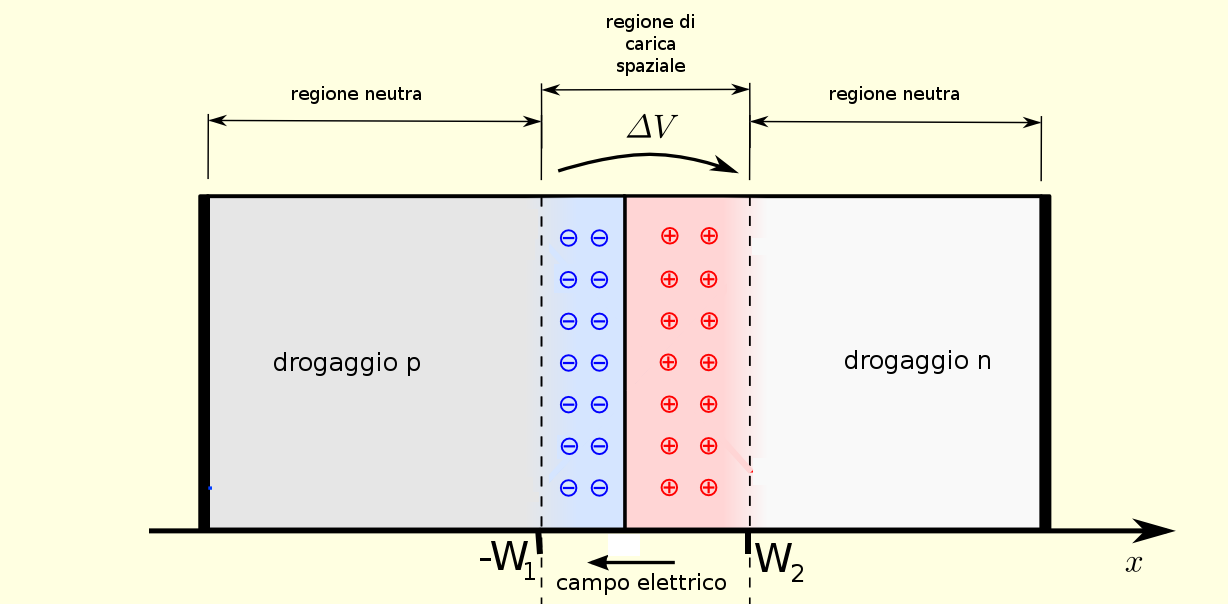
\includegraphics[height=0.5\textwidth]{res/cap 3/drogaggio}
    \caption{Rappresentazione di semiconduttore con drogaggio p-n}
\end{figure}\noindent
Si formano quindi due zone, la prima con una prevalenza di elettroni liberi e la seconda con lacune le quali provocano una carenza di elettroni andandosi a creare un campo elettrico che si estende a cavallo della regione di svuotamento.
Grazie al fenomeno illustrato in precedenza se si illumina la giunzione dalla parte n vengono a crearsi delle copie elettrone-lacune in entrambe le zone, il campo elettrico presente a causa del drogaggio fa si che gli elettroni in eccesso si dividano e li spinge in direzioni opposte, una volta oltrepassata la regione di svuotamento non possono quindi più tornare indietro a causa della presenza del campo elettrico.\\
Procedendo quindi con una connessione sterna si otterrà un circuito chiuso nel quale il flusso di elettroni parte dallo strato n,a potenziale maggiore, per dirigersi nello strato p, a potenziale minore fintanto che la cella rimanere esposta ai raggi solari.\\
\subsection{Cella solare}
Una cella solare è un dispositivo elettrico a stato solido il quale tramite l'effetto fotovoltaico permette di convertire l'energia trasportata dalla luce solare in elettricità tramite l'effetto illustrato nella sezione precedente.\\
La maggior parte delle celle fotovoltaiche prodotte, se esposte al sole, producono una tensione di circa 0.6V, è quindi necessario metterle in serie per ottenere tensioni più alte.
Collegando le celle in serie però non si ha il controllo sulle singole celle in quanto la stessa corrente attraversa tutte le celle, quelle poste in ombra quindi finiscono per fare da strozzatura per tutto il sistema andando a scaldarsi e potenzialmente a danneggiarsi.\\
E' quindi visibile l'importanza di posizionare correttamente i pannelli fotovoltaici in modo che vi siano me zone d'ombra e per meno periodi possibili.\\
\subsection{Pannello fotovoltaico}
\paragraph{Struttura}\mbox{}\\
Un pannello fotovoltaico è formato da un'insieme di celle opportunamente collegate tramite una griglia metallica che è presente sulla superficie del modulo in modo da formare sia collegamenti in serie che in parallelo. Una volta collegate le celle si procede con l'assemblaggio del modulo ponendo sopra la superficie posteriore, realizzata con un materiale isolante con scarsa dilatazione termica,uno strato di acetato di vinile(EVA),si pone quindi lo strato di celle solare opportunamente collegate per poi porre un'ulteriore strato di EVA ed il vetro temperato a protezione dell'intero modulo.\\
\begin{figure}[H]
    \centering
    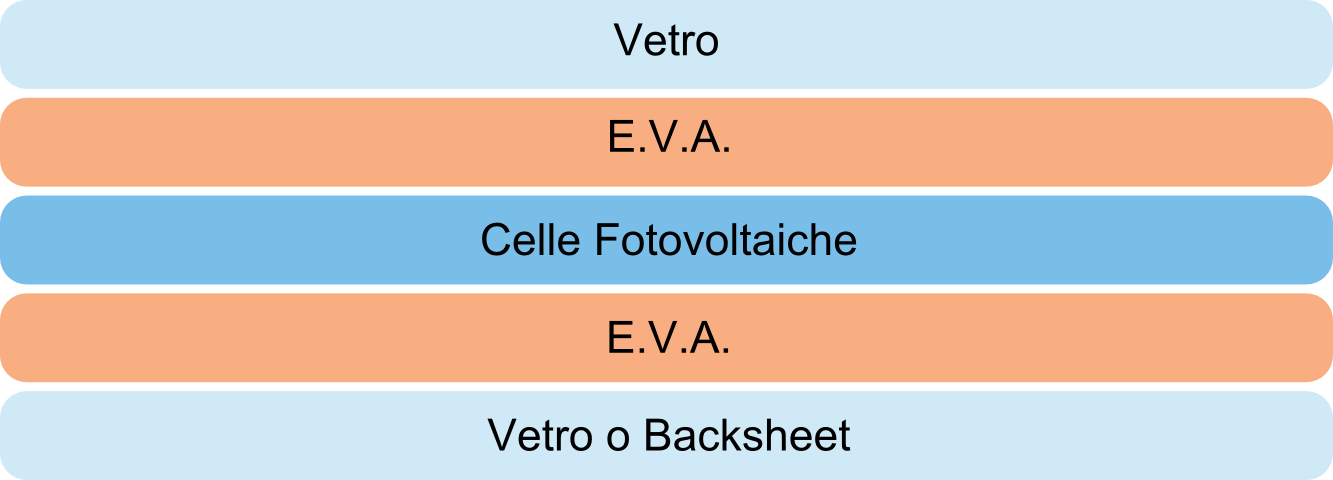
\includegraphics[height=0.3\textwidth]{res/cap 3/composizione modulo}
    \caption{Schema di composizione di un modulo fotovoltaico}
\end{figure}\noindent
Una volta assemblato si procede con un processo di pressofusione atto a trasformare l'EVA in un collante inerte, si collega la griglia ad una morsettiera che viene posta sul retro e si chiude il modulo in un frame di alluminio che faciliterà l'installazione e l'orientamento.
\paragraph{Tecnologie realizzative}\mbox{}\\
Dei molti semiconduttori utilizzabili per la produzione dei moduli fotovoltaici il più comunemente usato è il silicio, esso si ottiene in wafer che successivamente vengono uniti tra loro a formare un modulo.\\
Esistono diverse tipologie costruttive delle celle, tra le più comuni troviamo:
\begin{description}[labelindent=5mm]
    \item[$\cdot$ Silicio monocristallino:] ogni cella è realizzata a partire da un wafer formato da un monocristallo opportunamente drogato. Sono tendenzialmente costose perchè risulta difficile formare ampie superfici senza sprecare materiale o spazio però permettono di raggiungere un'efficienza dell'ordine del 18-21\%.
    \item[$\cdot$ Silicio policristallino:] in questo caso la cella è formata da un policristallo, quindi non strutturalmente omogeneo ma organizzato in grani localmente ordinati. Il costo in questo caso data la peggior qualità del silicio usato risulta più basso a favora di una maggior facilità di taglio e lavorazione. L'efficienza raggiungibile con questa tipologia di silicio però è più bassa del caso precedente e si attesta nell'ordine del 15-17\%. 
    \item[$\cdot$ Silicio amorfo:] questa tipologia di celle hanno un'efficienza più bassa ($\sim8\%$) ma risultano molto più economici da produrre rispetto ad i precedenti. Il silicio amorfo ha un bandgap più ambio dei precedenti(circa un 55\% in più) il che favorisce l'assorbimento della parte visibile dello spettro solare ma risulta meno efficiente nell'elaborare la parte infrarossa.
\end{description}
\paragraph{Prestazioni ed efficienza}\mbox{}\\
Le prestazioni offerte dal singolo modulo dipendono da diversi fattori, in prima approssimazione si può calcolare la potenza che un pannello è in grado di esprimere con la seguente formula:
\begin{center}
    \large{$P = \eta I_0 S \sin(\alpha)  $}
\end{center}
Dove con $I_0$ considero l'irradianza perpendicolare alla superficie, con S la superficie del modulo, mentre $\alpha$ è l'angolo che il modulo ha con il sole, $\eta$ invece è un fattore di rendimento.\\
In conclusione possiamo osservare come i parametri fisici che influenzano la produzione di un pannello solare possano essere sintetizzati in:
\begin{itemize}
    \item Irraggiamento a cui il pannello è esposto
    \item Angolo con la quale in modulo è orientato
    \item Qualità produttiva del modulo
    \item Tipologia di silicio usato
\end{itemize}
Si nota anche qui l'importanza di collocare il pannello in una regione che abbiamo una buona copertura da parte del sole ed in una superficie correttamente orientata.\\
Nel caso di installazioni su tetti questi due parametri rendono o meno un determinato tetto idoneo all'installazione, nel caso si installino in campi fotovoltaici invece l'angolo di installazione
viene scelto in fase costruttiva quindi ideale per il luogo in cui è collocato.\\
Come visto in precedenza l'angolo con cui la luce solare colpisce la terra dipende sia dal luogo geografico che dal periodo dell'anno preso in esame,
vi sarà quindi un'efficienza diversa da periodo data dall'inclinazione del modulo oltre che dalle condizioni climatiche.\\
Il singolo modulo in condizioni normali lavora in un range di tensione a vuoto($V_{OC}$) tra 40 ed i 50 Volt ed una corrente di cortocircuito($I_{sc}$) tra i 9 ed i 12 Ampere.\\
Un'altro fattore importante che influenza negativamente il rendimento di un pannello fotovoltaico è la temperatura,
infatti la temperatura della giunzione p-n va ad influenzare sia ($V_{OC}$) che ($I_{sc}$) andando quindi ad alterare anche la potenza massima($P_{Max}$) che il modulo è in grado di offrire.\\
Per quantificare l'impatto della temperatura sul pannello ogni produttore fornisce tre valori tre espressi in $\frac{\%}{^\circ C}$:
\begin{enumerate}
    \item Coefficiente di temperatura di ($P_{Max}$)
    \item Coefficiente di temperatura di ($V_{OC}$)
    \item Coefficiente di temperatura di ($I_{sc}$)
\end{enumerate}
\paragraph{Dati sperimentali}\mbox{}\\
Prendendo un modulo come esempio possiamo vedere
